\documentclass[a4paper, 11pt]{report}

%%%%%%%% FRONT MATTER %%%%%%%%
\usepackage[margin=1in]{geometry}
\usepackage[colorlinks=true, pdfstartview=FitV, linkcolor=black, 
            citecolor=black, urlcolor=blue]{hyperref}

\usepackage{titlesec}
\titleformat{\chapter}[hang] 
{\normalfont\huge\bfseries}{\thechapter:}{1em}{} 

\usepackage{amsmath, amssymb}

\usepackage{xcolor}
\definecolor{LightGray}{gray}{0.9}

\usepackage{fancyvrb}
\DefineVerbatimEnvironment{verbatim}{Verbatim}{xleftmargin=.2in, frame=single}
\makeatletter
\renewcommand*\verbatim@nolig@list{}
\makeatother

\usepackage{tabularx}
\usepackage{cprotect}


\usepackage{fontspec}
\setmainfont[
 BoldFont={Lato Regular},
 ItalicFont={Lato Light Italic},
 BoldItalicFont={Lato Italic}]{Lato Light}
\setmonofont{JetBrainsMonoNerdFont}[Contextuals=Alternate, Scale=0.8]
\newfontfamily\mainthick{Lato}

\usepackage{minted}
\setminted{
fontsize=14pt,
frame=single,
framesep=2mm,
fontsize=\footnotesize,
xleftmargin=0.5in,
xrightmargin=0.5in,
linenos,
autogobble,
breaklines
}
% \usepackage{lstlistings}
\pagenumbering{arabic}
\pagecolor{white}

\setcounter{secnumdepth}{3}
\setcounter{tocdepth}{3}


\usepackage{tikz}
\usepackage{pgfplots}

\newenvironment{greytext}{\color{LightGray}}{\ignorespacesafterend}

\begin{document}

\newcommand{\coderef}[2]{(\ref{#1}\ l.#2)}
\newcommand{\comment}[1]{}

%!TEX root = nea-final.tex

\begin{titlepage}
\vspace*{1cm}
\begin{center}

{\mainthick
\Huge\noindent\textbf{The Lilac Programming Language}
}

\vspace{12pt}
\par\noindent\rule[12pt]{96pt}{0.8pt}\\
\LARGE
Language Design and Interpreter Implementation

\normalsize
\vspace{5cm}

\par\noindent\rule[12pt]{96pt}{0.8pt}\\
\begin{tabularx}{0.8\textwidth} {
		>{\raggedleft\arraybackslash}X
   		>{\raggedright\arraybackslash}X }
\textbf{Name:} & :3\\ %Éloi Thibault\\
\\
\textbf{Candidate Number:} & 3253\\
\\
\textbf{Centre Number:} & 14613\\
\end{tabularx}\\
\vspace{12pt}
\par\noindent\rule[12pt]{96pt}{0.8pt}\\
\end{center}

\vspace*{\fill}
\textbf{Orleans Park School}
\end{titlepage}
\newpage

\tableofcontents
\newpage

\chapter{Analysis}\label{sec:analysis}
\section{Introduction}\label{sec:introduction}

For my A-level project I am going to design and implement a small programming language, called Lilac. In the world of programming languages, there are the big production languages: Python, JavaScript, C++, C\#, etc. While they are the most commonly used languages, they are by no means the only ones. On the outskirts of the field of language design, there are many small languages which seek to either push the boundaries of computation and abstraction, or that have incredibly specific applications (along with, of course, the ones written as jokes). For example, the \verb|Orca| language is a two-dimensional graphical language which is designed for programmatic music production. \verb|Pinecone| was another attempt at creating a light c-style language. And most commonly formats such as \verb|toml| and \verb|yaml| that are used for configuration files lean gently into the most minimal of language. To summarise, wherever there could be an issue with one of the large languages, there are small languages being designed to try to fix it.\\
\\
I see Lilac in this way. The issue that it is trying to solve is the accessibility of functional programming. Haskell, the giant of the paradigm, is incredibly difficult to learn because it is a huge jump in abstraction and type theory. But often the functional approach to problem solving is the most efficient, and it is an incredibly powerful paradigm. My motivation for this project is to create an intermediary language, a solution that is genuinely functional, but not overwhelming for a first-time functional programmer. As such, the type system should be loose, and I take some liberties with the strictness of functions. But at the core of it, it is a language strongly inspired by lambda calculus, and the aim is that learning Lilac would solidly introduce the concepts necessary for functional programming.\\
\\
\section{Translator Design}\label{sec:translator-design}
A translator is a piece of utility software that takes one set of program source code and turns it (translates) into the program source code of another language. They are incredibly versatile pieces of software, and as such there are many different ways of desinging and implementing translators. Generally, they come in three different forms. Most basic are assemblers, which take assembly language code and translate it to executable machine code. Then, we have interpreters and compilers, which translate high level languages. These are significantly more complicated, since they also have to take into account the code semantics and structure. Interpreters and compilers differ generally in their output. And interpreter translates line by line (or construct by construct) and executes as it goes, stopping when it reaches a halting condition; this could be an error or just the end of the code. Compilers translate the entire source code and output an executable machine code file. It always stops when it reaches the end, forming a list of errors as it goes.\\
\\
Although interpreters and compilers have separate outputs, they follow very similar steps. The way that these steps are connected, so the path that the data takes, is part of what gives each language and translator its individual flavor.\\
\\
\begin{figure}[ht]
\centering
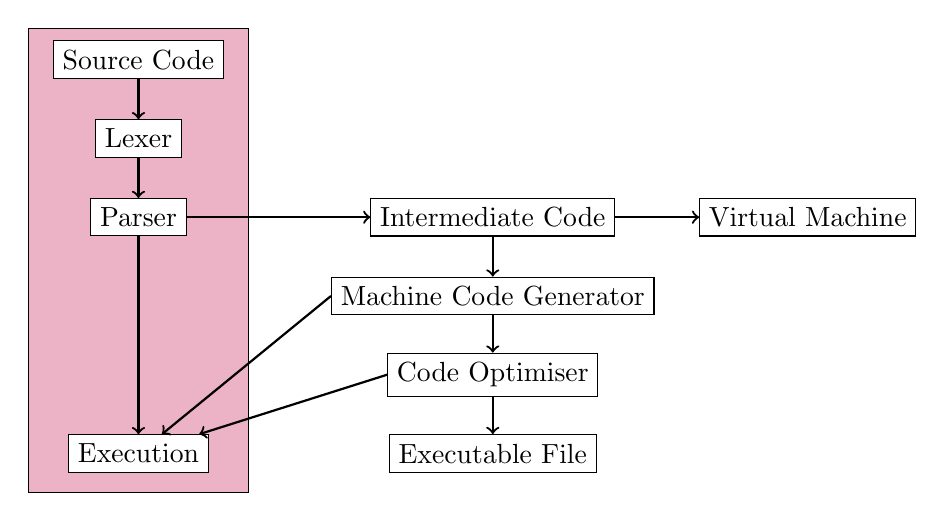
\begin{tikzpicture}
  \draw[fill=purple!30] (-1.4, 0.4) -- (1.4, 0.4)-- (1.4, -5.5) -- (-1.4, -5.5) -- (-1.4, 0.4);
  
  \node[rectangle, fill=white, draw] (source) at (0,0) {Source Code};
  \node[rectangle, fill=white, draw] (lexer) at (0,-1) {Lexer};
  \node[rectangle, fill=white, draw] (parser) at (0,-2) {Parser};
  \node[rectangle, fill=white, draw] (execution) at (0,-5) {Execution};
  \node[rectangle, fill=white, draw] (inter) at (4.5,-2) {Intermediate Code};
  \node[rectangle, fill=white, draw] (codegen) at (4.5,-3) {Machine Code Generator};
  \node[rectangle, fill=white, draw] (optimiser) at (4.5,-4) {Code Optimiser};
  \node[rectangle, fill=white, draw] (execfile) at (4.5,-5) {Executable File};
  \node[rectangle, fill=white, draw] (vm) at (8.5,-2) {Virtual Machine};
  
  \draw[thick, ->] (source) -- (lexer);
  \draw[thick, ->] (lexer) -- (parser);
  \draw[thick, ->] (parser) -- (execution);
  \draw[thick, ->] (parser) -- (inter);
  \draw[thick, ->] (inter) -- (codegen);
  \draw[thick, ->] (codegen) -- (optimiser);
  \draw[thick, ->] (optimiser.west) -- (execution);
  \draw[thick, ->] (codegen.west) -- (execution);
  \draw[thick, ->] (optimiser) -- (execfile);
  \draw[thick, ->] (inter) -- (vm);
\end{tikzpicture}
\label{fig:translator-graph}
\caption{Graph showing the possible steps a translator might take.}
\end{figure}
\\
Figure \ref{fig:translator-graph} shows the steps a translator could take when executing a piece of program source code. The section in the purple box is what my project is limited to. The first two stages are common to all translators. The lexer performs lexical analysis on the source code. This turns the input text into a list of tokens. At their simplest, tokens are just simple pairs that each represent one semantic component of the source code. In programming, the line of code \verb|var: 3| would be turned into \verb|[(Identifier, 'var'), (Assi| \verb|gnment, ':'), (Number, 3)]|. At this point, errors can already be caught. For example, if an identifier does not start with a letter or if an illegal symbol is used, the lexer will catch this. If we introduce an example from english, the sentence "The cat likes to sleep" is composed of different types of words. The lexer would be where we notice that "Teh cta ilkse ot eples" is not an allowed sentence in english, since none of the words are allowed. However, the lexer would not notice that "cat to the sleep likes" is not an allowable sentence.\\
\\
Now, the source code is represented as a flat list of tokens. However this list does not have any grammatical structure. Adding this structure is the next step, called parsing. The result is a parse tree or abstract syntax tree, a tree data structure which represents the grammatical structure of a string. This is where operator precedence and associativity becomes apparent, and differentiates \verb|(3+2)*4| from \verb|3+(2*4)|. Here, grammatical errors are noticed. If I use the assignment operator with nothing on one side, this is noticed as an error. To use the english example, the parser would notice that "cat to the sleep likes" should not be allowed as an english sentence, because the order of word types does not follow the rules of the grammar. For "the cat likes to sleep", the parse tree may look like Figure \ref{fig:cat-likes-sleep}. Notice that the syntactic rules of the English grammar are implied as subtrees of the overall parse tree. This same idea applies to programming languages; for a simple line of code in Lilac like \verb|var: 4 * (2 + 3)| the tree would look like Figure \ref{fig:lilac-tree-example}.
\\

%\verb|Missing Pasted image 20221026100107.png|500|\\
\begin{figure}[ht]
\centering
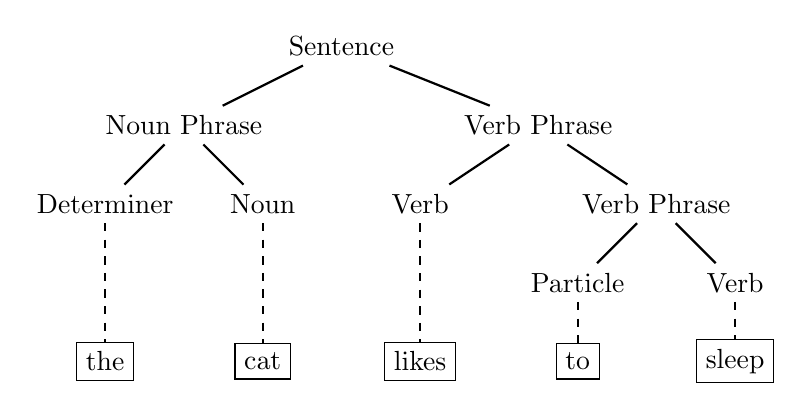
\begin{tikzpicture}
  \node[rectangle] (s) at (0,0) {Sentence};
  \node[rectangle] (np) at (-2,-1) {Noun Phrase};
  \node[rectangle] (det) at (-3,-2) {Determiner};
  \node[rectangle] (n) at (-1,-2) {Noun};
  \node[rectangle, draw] (the) at (-3,-4) {the};
  \node[rectangle, draw] (cat) at (-1,-4) {cat};
  
  \node[rectangle] (vp) at (2.5, -1) {Verb Phrase};
  \node[rectangle] (verb) at (1,-2) {Verb};
  \node[rectangle] (vp2) at (4, -2) {Verb Phrase};
  \node[rectangle] (p) at (3,-3) {Particle};
  \node[rectangle] (verb2) at (5, -3) {Verb};
  \node[rectangle, draw] (likes) at (1,-4) {likes};
  \node[rectangle, draw] (to) at (3,-4) {to};
  \node[rectangle, draw] (sleep) at (5,-4) {sleep};

  \draw[thick] (s) -- (np)
  	           (s) -- (vp)
               (np) -- (det)
               (np) -- (n)
               (vp2) -- (p)
               (vp2) -- (verb2)
               (vp) -- (verb)
               (vp) -- (vp2);
               
  \draw[thick, dashed]
               (det) -- (the)
               (verb) -- (likes)
               (n) -- (cat)
               (p) -- (to)
               (verb2) -- (sleep);
\end{tikzpicture}
\caption{English parse tree of the sentence "the cat likes to sleep"}
\label{fig:cat-likes-sleep}
\end{figure}

\begin{figure}[ht]
\centering
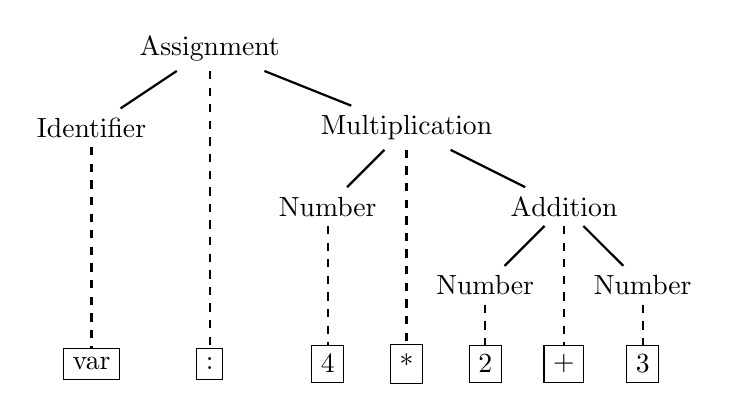
\begin{tikzpicture}

\node[rectangle] (assign) at (0,0) {Assignment};
\node[rectangle] (id) at (-1.5,-1) {Identifier};
\node[rectangle] (mult) at (2.5,-1) {Multiplication};
\node[rectangle] (num4) at (1.5,-2) {Number};
\node[rectangle] (add) at (4.5,-2) {Addition};
\node[rectangle] (num2) at (3.5,-3) {Number};
\node[rectangle] (num3) at (5.5,-3) {Number};
\node[rectangle, draw] (var) at (-1.5,-4) {var};
\node[rectangle, draw] (colon) at (0,-4) {:};
\node[rectangle, draw] (four) at (1.5,-4) {4};
\node[rectangle, draw] (star) at (2.5,-4) {*};
\node[rectangle, draw] (two) at (3.5,-4) {2};
\node[rectangle, draw] (plus) at (4.5,-4) {+};
\node[rectangle, draw] (three) at (5.5,-4) {3};

\draw[thick] (assign) -- (id)
             (assign) -- (mult)
             (mult) -- (num4)
             (mult) -- (add)
             (add) -- (num2)
             (add) -- (num3);

\draw[thick, dashed] (id) -- (var)
             (assign) -- (colon)
             (num4) -- (four)
             (mult) -- (star)
             (num2) -- (two)
             (add) -- (plus)
             (num3) -- (three);
\end{tikzpicture}
\caption{An example parse tree for Lilac}
\label{fig:lilac-tree-example}
\end{figure}

Notice that in this in this tree the parentheses are not included. Instead, they are used to specify subtrees of the overall parse tree. If I wrote \verb|4 * 2 + 3|, the parser would realise that \verb|*| is first in the order of operations. It would therefore treat it as \verb|(4 * 2) + 3|, which produces a different tree. There is also another key difference between English and Lilac. Notice that in the programming language, every node of the tree has a token in the string associated, whereas in the english sentence this is not the case. Lilac is explicitly structured, or context-free. There is no way of making a string which can be parsed in more than one way.\\

There are several ways to define the grammar of a language, and the algorithms to parse it. A common method for defining a grammar is through production rules, usually written in a syntax called Backus-Naur Form. Here is an example, which defines arithmetic between integers and the order of operations:
% null null\\
\begin{verbatim}
<expr> ::= <expr> + <term>
         | <expr> - <term>
         | <term>

<term> ::= <term> * <factor>
         | <term> / <factor>
         | <factor>

<factor> ::= ( <expr> )
           | - <factor>
           | <int>

<int> ::= <int><digit>
     s   | <digit>

<digit> ::= 0 | 1 | 2 | 3 | 4 | 5 | 6 | 7 | 8 | 9
\end{verbatim}

The use of \verb|::=| defines a rule in the production, which is represented with an identifier within the angle brackets. For example, the rule \verb|<expr>| tells us that it is either an \verb|<expr>| followed by a \verb|+| symbol followed by a \verb|<term>|, or an \verb|<expr>| followd by a \verb|-| symbol followed by a \verb|<term>|, or just a \verb|<term>|. The repeated application of these rules can be used to determine whether a string of terminal characters (everything that is not \verb|::=|, \verb|\||, or in angle brackets) can be produced from this grammar. There is no way to make the string \verb|3+|, so this is not part of the language defined by the grammar. This sort of definition is used for context-free languages, where the syntax can always be represented by a set of deterministic rules. Parsing algorithms are generally divided in two categories. Top-down parsers start with the wider rules and then narrow down, while bottom-up parsers start with the terminals and build up a parse tree.\\

Execution is comparatively simpler. Most methods use a walk through the parse tree along with a call stack to execute the code. The call stack keeps track of the order in which sections of code should be executed. The individual pieces are wrapped in "stack frames" that seperate scope and pointers. For example, recursive function calls are protected by the stack frames so that the inner scopes do not overwrite the outer scope. After something is pushed to the call stack it can then be popped and executed in the correct order. If the interpreter is written in a low-level language the individual memory management of each operation has to be implemented. If it is written in a high-level language then the operations would be implemented in that same high level language.\\

\section{Proposed Solution}\label{sec:proposed-solution}

My proposed solution is called \verb|Lilac|. It is a minimal functional programming language inspired by the syntax of Pinecone and Boa, along with the function logic of Haskell. Here is an example source file:\\
% null null\\
\begin{verbatim}
main: ( print "Hello World" )

addToThree: ( fn x -> 3 + x )

fooBarBaz:
  let (
    byThree: n % 3,
    byFive: n % 5 )
  in (
    fn n -> byThree ? "Foo" | byFive ? "Bar" | "Baz" )
\end{verbatim}
\subsection{Language Specification:}\label{sec:language-specification}
\subsubsection{Types:}
Lilac has built in data types \verb|number|, \verb|string|, and \verb|boolean|, although these are mostly hidden from the user. Lilac is dynamically and weakly typed. The set \verb|number| is defined as all integers and floating point numbers, \verb|string| is the set of all character strings, and \verb|boolean| is the set \verb|{true, false}|.\\

\subsubsection{Operators:}
All the standard operators for numeric arithmetic, boolean arithmetic, logic and comparison are implemented:\\
% null null\\
\begin{verbatim}
Numbers: +, -, *, /, %
Boolean: &&, ||, !
Comparison: =, <, >, <=, >=, != (! =)
\end{verbatim}

\subsubsection{Variables:}
Variables are created when a value is assigned to a name using the \verb|:| operator. Lilac evaluates lazily, which means that it does not evaluate any expressions untill the point where the value is needed. This means that you could define the variable \verb|x: 3 + 2|, and it will be kept in memory as the expression $3+2$ until x is referenced. This is unlike eager evaluation where the value of \verb|x| is immediately calculated on assignment.

In Lilac everything is also a first-class citizen, which means that practically any expression (other than an assignment) can be assigned to a variable or passed to and from a function.

\subsubsection{Conditionals:}
Lilac uses a ternary operator syntax for an if-then-else statement. The statement "if x then y else z" is \verb|x ? y | z|. Of course, \verb|z| could be another conditional expression; if \verb|z: a ? b | c|, the statement becomes \verb|x ? y | a ? b | c|, or in natural language "if x then y else if a then b else c". From an evaluation point of view, conditional expressions aren't staatements or control structures, but operators that evaluate to values. So, our first example \verb|x ? y | z| is equivalent to \verb|y| if \verb|x| is true. This means a variable can have a conditional value.

\subsubsection{Functions:}
The syntax for function defintion is inspired by lambda expressions in haskell and python:\\
% null null
\begin{verbatim}
Haskell:
	(\x -> x + 2)
Python:
	(lambda x: x + 2)
Lilac:
	( fn x -> x + 2 )
\end{verbatim}

The label \verb|fn| is explicitly required to show that it is a function (in the future there is the possibility of adding different varieties). A function can be treated as a block which is assigned to a variable, or a lambda which is directly applied to a value, or again as a first class citizen that is returned from another function. Function application uses a blank whitespace as the operator. Crucially, this is left associative. Consider this example:
% null null
\begin{verbatim}
add: ( fn x -> ( fn y -> x + y ))
add 3 2 = (add 3) 2 = 5
\end{verbatim}

The second line is true because of the left associativity of the whitespace operator. \verb|(add 3)| returns a function which is applied to \verb|2|. The operator \verb|;| can be used to change the direction of associativity, similarly to parentheses:\\
% null null
\begin{verbatim}
print add 3 2 = (((print add) 3) 2) (Error because (print add) does not return a function)
print;add 3 2 = (print ((add 3) 2))
\end{verbatim}

\subsubsection{Let-In expression:}
This expression is inspired from mathematical literature where the values in an expression are often specified in the following way:\\

\[ \text{let}\ a=2\ \text{and}\ b=3\ \text{in}\ \sqrt{a^2+b^2} \]

In Lilac, it can be helpful to be able to break up a function into temporary definitions. It could be done in the following way:\\
% null null\\
\begin{verbatim}
divBy:
  ( fn n -> ((fn x -> x % 3) n = 0 ? "Three" | 
             (fn x -> x % 5) n = 0 ? "Five" | "Other" ))

divBySimpler:
  let 
    ( byThree: ( fn x -> (x % 3) = 0 ),
      byFive:  ( fn x -> (x % 5) = 0 ))
  in
    ( fn n -> byThree n ? "Three" | byFive n ? "Five" | "Other" )
\end{verbatim}
\section{Objectives}\label{sec:objectives}
By the end of this project I aim to have written an interpreter for the Lilac programming language which can:\\
\begin{itemize}
\item 
Execute arithmetic
\item 
Execute boolean arithmetic and comparison
\item 
Define and store variables
\item
Define and use functions
\item 
Conditional statements
\item 
Recursive function calls and definitions
\end{itemize}

In addition to this, the interpreter should provide a REPL and the ability to run source files. It should also be able to import files into the REPL or another script. This should also be accessible from a shell script.

\chapter{Design}\label{sec:design}
\section{Stage One: Framework and Interface}\label{sec:stage-one-framework-and-interface}
I start with a driver class called \verb|Lilac|. This will contain all the interactive elements of the interpreter, and drive the execution. The class will expose the useful functions \verb|runFile|, \verb|runLine|, both of which take a simple string of text and then execute it as lilac. It also provides a REPL functionality that can provides an interactive output as shown here:\\
% null null
\begin{verbatim}
Lilac Interactive Mode

<i> str: "hello"
<i> length str
<o> 5
<i> f:
  >   let ( y: length str )
  >   in ( fn n -> y + n )
<i> x + f 3
<e> [Line 1] NameUndefinedError: The name 'x' does not exist in this scope
\end{verbatim}
\subsection{Error Reporting}\label{sec:error-reporting}
It is crucial that my project implements some kind oferror checking and reporting. There are many errors that a user could make, and each should be differentiated and handled. There needs to be some kind of enumerable which keeps track of all the error types. It will look as follows:

\begin{verbatim}
enum ErrorType:
	SyntaxError
	NameUndefinedError
	ArgumentError
	TypeError
\end{verbatim}

These will be used in conjunction with Lilac's \verb|error| method. This will take an error type, a line number, and a message about the error to print. 

\section{Stage Two: Lexical Analysis}\label{sec:stage-two-lexical-analysis}
The lexer is represented by a Lexer class:

\begin{verbatim}
class Lexer:
    tokens :: List[Tokens]
    source :: String

    scan :: method
    add_token :: method
    match_next :: String -> bool
    peek :: method -> String
    is_alpha :: String -> bool
    is_num :: String -> Bool
\end{verbatim}

The scan method implements the scanning algorithm. This takes the source code as a string and loops through it. The algorithm is as follows:
% null null\\
\begin{verbatim}
while not at the end of the source:
    character = consume the next character
    match on character:
        if it represents a single charcter token:
            add token(character)
        if it can start a two character token:
            check the next character without consuming
            add token(both characters)
        otherwise:
            add token representing a number or identifier
            or throw an error
\end{verbatim}
This algorithm deals with characters that can form multiple tokens (like \verb|<|and \verb|<=|) by cautiously looking ahead at the next character. If the scanner detects an alphanumeric character, it moves to the state of scanning a number, identifier, or string. It does this by continuing to advance until certain criteria are met. For a number, it keeps going until the next character is not a digit, but one period is allowed in the number. If there is a period, then the number is a float, otherwise it is an int.

\section{Stage Three: Parsing}\label{sec:stage-three-parsing}
In parsing, I seek to translate the list of tokens that the Scanner outputs into a tree data structure. I decide to use a recursively defined tree in order to optimise the simplicity and dynamicity of the structure definition. The tree type is defined as follows:\\
% null null
\begin{verbatim}
class Tree:
	token :: Token
	action :: Action
	left :: Tree
	right :: Tree

	is_leaf :: Tree -> boolean
\end{verbatim}

The parser uses a recursive, functional approach:
% null null\\
\begin{verbatim}
function to_tree(tokens: list of tokens):
	if there is still at least one operator in the source:
		index = find position of the lowest precedence operator
		action = make a new action corresponding to this operator
		
		left_expr = all tokens to the left of index
		right_expr = all tokens to the right of index
		operator = element of tokens at index
		
		clean outer parentheses from the left and the right
		
		left_tree = to_tree(left_expr)
		right_tree = to_tree(right_expr)
		return a Tree with operator, action, left_tree, right_tree
		
	otherwise:
		action = make a new literal action
		return a Tree with operator, action
\end{verbatim}

To find the position of the operator with the lowest precedence, I need a table defining precedence and associativity. Figure \ref{fig:operator-table} shows the rules that I make for lilac, inspired by the operator rules for \verb|Haskell| and \verb|C|. When finding the index, the algorithm should ignore expressions in parentheses, as these are guaranteed to be subtrees. Cleaning the parentheses from an expression simply means turning \verb|(2*3)| into \verb|2*3|; parentheses are only important for parsing, and should themselves not be parsed. The associativity of the operator describes the direction in which it should be parsed if there are multiple identicaloperators in a row. For example, addition is given right associativity, which means \verb|a + b + c| is understood as \verb|(a + (b + c))|. Notice, for example, that function application is left associative, but the semi-colon is right associative. Both of these "do the same thing", but in opposite directions. Conditional statements also need to be carefully considered. In the complex statement \verb{a ? b | c ? d | e{, we first want \verb|a| to be tested, then to either do \verb|b| or test \verb|c|. The expression shoul be parsed like this: \verb{(((a?b)|(c?d))|e){, which means pipe has to be left associative so that the first conditional is put prior in the order.
\begin{figure}[ht]
\centering
\begin{tabular}{c|c c}
Token Type & Precedence & Associativity\\
\hline\\
Colon (\verb|:|) & 0 & Right \\
Space ( ) & 10 & Left \\
Arrow (\verb|->|) & 1 & Right \\
Pipe (|) & 2 & Left \\
Question (\verb|?|) & 2 & Right \\
Semi-colon (\verb|;|) & 3 & Right \\
Slash (\verb|/|) & 8 & Right \\
Star (\verb|*|) & 8 & Right \\
Plus (\verb|+|) & 7 & Right \\ 
Minus (\verb|-|) & 7 & Right \\
Equal (\verb|=|) & 6 & Right \\
Less (\verb|<|) & 6 & Right \\
Greater (\verb|>|) & 6 & Right \\
Less or equal (\verb|<=|) & 6 & Right \\
Greater or equal (\verb|>=|) & 6 & Right \\
Or (\verb||||) & 5 & Right \\
And (\verb|&&|) & 4 & Right \\
\end{tabular}
\caption{Operator table which defines the syntax of Lilac}
\label{fig:operator-table}
\end{figure}

\section{Stage Four: Execution}\label{sec:stage-four-execution}
\subsection{Execution model: The Tree Machine}\label{sec:execution-model-the-tree-machine}
The parser, thanks to my design of Lilac, outputs a recursive binary parse tree. At this point there are a few ways to proceed with execution. I considered doing a post-order traversal, and then using a simple stack/virtual machine. However, it is difficult to implement code branching and lazy evaluation this way. This is due to the fact that it is a bottom up technique, so at the leaves of the tree it is completely unaware of the context above it. Instead, I decide to manipulate the AST directly, and to execute it recursively in a top down manner. This is handled by my driving class, the \verb|TreeMachine|. It is defined as follows:\\
% null null\\
\begin{verbatim}
TreeMachine:
    env_monad :: EnvMonad
    tree :: Tree
    
    execute :: Tree -> (*output)
\end{verbatim}

The TreeMachine is the object that is responsible for running the code. In the REPL context it will only do the execute function on one line, but in a script context it will also handle imports, (running the machine on another source file while ignoring main), and running \verb|main|.\\

\subsection{Monads: Stack}\label{sec:monads-stack}
A central issue in my design is deciding where behaviours go, and who handles what. To solve this, I decide to opt for a monadic model. A monad is an object that contains some value, and handles behaviors and side effects relating to that value. This is helpful for separating behavior from types, and to improve the simplicity of the code. For example, the \verb|Maybe| monad allows for safe computation. The data stored within it can be either \verb|Just x| or \verb|Nothing|. If a computation fails, the monad catches this and makes the value \verb|Nothing| - our computation is saved. The two main components of a monad are the \verb|return| function and the \verb|bind| function. Borrowing the type signatures from haskell, these look like:
% null null\\
\begin{verbatim}
return :: Monad m => a -> m a
bind (>>) :: Monad m => m a -> (a -> m b) -> m b
\end{verbatim}

Here we see that \verb|return| takes a value of type \verb|a| and returns a monad containing a value of type a. In an object-oriented way, this is the class constructor. We also see that bind, which also has the operator \verb|>>| takes a monad of type \verb|a| and a function that returns a monad of type \verb|b|, then returns a monad of type \verb|b|. Simply, it takes a monad, applies the function to the value inside the monad, then returns the output from that. This is the central benefit of the monad; the behavior is completely separate from the value.\\

For my call-stack, which is used to evaluate expressions, I use this model. I create three classes: \verb|Stack|, \verb|Node|, and \verb|StackMonad|. The stack is defined in a dynamic linked way using the \verb|Node| class in the following way:
% null null\\
\begin{verbatim}
class Node:
    value :: Token
    next :: Node

class Stack:
    top :: Node
    
    pop :: Stack -> Stack
    push :: Stack -> Token -> Stack
\end{verbatim}

Then, I define the \verb|StackMonad| like so:
% null null
\begin{verbatim}
class StackMonad
    stack :: Stack
    out :: List[Tokens]
    
    (>>) :: StackMonad -> function -> StackMonad
\end{verbatim}

The functions that bind will take are the stack operations, and bind will simply run them. The output of popping the stack is stored in the \verb|out| list of the monad.\\
\subsection{Monad: Environment and Actions}\label{sec:monad-environment-and-actions}
I have an \verb|Environment| class, which can also be thought of as a scope. This class looks as follows:
% null null\\
\begin{verbatim}
class Environment:
    stack_monad :: StackMonad
    table :: Dictionary
    tree :: Tree (optional)
\end{verbatim}

We can see here that the environment holds only data, and no behaviors. It is contained within my \verb|EnvMonad| class:
% null null\\
\begin{verbatim}
class EnvMonad:
    env :: Environment
    trace :: List
    
    bind (or >>) :: EnvMonad -> Action -> EnvMonad
    consume :: EnvMonad -> Environment -> EnvMonad
\end{verbatim}

The \verb|bind| function is a feature of monads. It takes an \verb|EnvMonad| (i.e. self) and an \verb|Action|, runs the action on the data of the monad, then returns the result wrapped in a new monad. The \verb|Action| is a function wrapped in a class:
% null null\\
\begin{verbatim}
class Action:
    left :: Tree
    right :: Tree
    run :: Environment -> Environment
    check :: (*args) -> (*outputs)
\end{verbatim}

Each component of the language gets its own action, and the interface for each action is strictly the same. This allows me to easily extend the language, simply by adding new actions. Each action has a reference to the left and right subtree of its parent node. Execution is done top-down: before an action executes itself, it does the left action and the right action. So, the run algorithm looks like:

\begin{verbatim}
run(envmonad):
    envmonad >> left action >> right action
    get any output
    check the arguments for the action
    do the action
\end{verbatim}

Since actions are kept in classes, I can use inheritance to approximate the idea of typeclasses. I'll make the \verb|Action| class generic, and then have other actions inherit from it. For example, the \verb|ArithmeticAction| will implement the \verb|check| method so that it make sures the left and right operands are numbers. Then thte actions for addition, multiplication, etc. will inherit from \verb|ArithmeticAction| and will be able to use the specific check method. This also means I can do general type checks on actions. The action pushes its result to the stack inside a \verb|Token|, and while it does the calculation. The stack is used as the intermediate structure where data is passed between actions and kept in order.

\section{Example}

To understand how my design works, let's imagine the simple example \verb|var: 3 + 4|. The scanner understands this as \mintinline{latex}{[(IDENTIFIER, var), (COLON, :), (NUMBER, 3), (PLUS, +), (NUMBER, 4)]}. Then, the parser parses this and gives it the structure show in Figure \ref{fig:example-tree}. This structure is translated into an action tree (which lives, polymorphically, on the same tree rather than on a new instance). This structure is then passed for execution. To begin with, the action of the root node is executed (\verb|AssignAction|). This executes the action of its left subtree and its right subtree, then itself. The left subtree is an \verb|IdentifierAction|, which represents a terminal. It pushes \verb|var| to the stack (Figure \ref{fig:example-stack}.1), then returns. The 

\begin{figure}[ht]
\centering
\begin{tabular}{|c|c|}
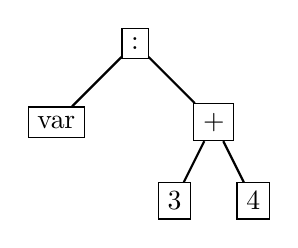
\begin{tikzpicture}

\node[rectangle, draw] (assign) at (0,0) {:};
\node[rectangle, draw] (id) at (-1,-1) {var};
\node[rectangle, draw] (add) at (1,-1) {+};
\node[rectangle, draw] (num3) at (0.5,-2) {3};
\node[rectangle, draw] (num4) at (1.5,-2) {4};

\draw[thick] (assign) -- (id)
             (assign) -- (add)
             (add) -- (num4)
             (add) -- (num3);
\end{tikzpicture}
&
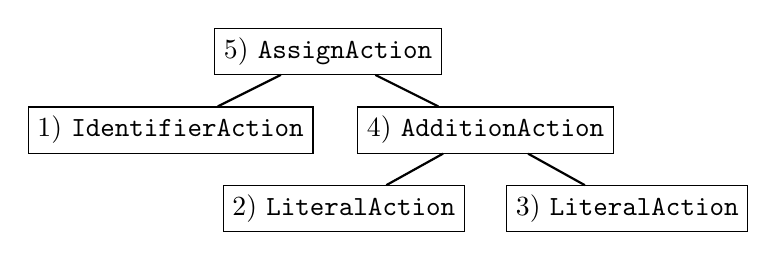
\begin{tikzpicture}

\node[rectangle, draw] (assign) at (0,0) {5) \verb|AssignAction|};
\node[rectangle, draw] (id) at (-2,-1) {1) \verb|IdentifierAction|};
\node[rectangle, draw] (add) at (2,-1) {4) \verb|AdditionAction|};
\node[rectangle, draw] (num3) at (0.2,-2) {2) \verb|LiteralAction|};
\node[rectangle, draw] (num4) at (3.8,-2) {3) \verb|LiteralAction|};

\draw[thick] (assign) -- (id)
             (assign) -- (add)
             (add) -- (num4)
             (add) -- (num3);
\end{tikzpicture}
\end{tabular}
\label{fig:example-tree}
\cprotect\caption{The parse tree for \verb|var: 3 + 4|, as a symbol tree and an action tree.}
\end{figure}

\begin{figure}[ht]
\centering
\begin{tabular}{c c c}
  1) \verb|IdentifierAction(var)| & 2) \verb|LiteralAction(3)| & 3) \verb|LiteralAction(4)|\\
  \begin{tabular}{c|c}
    Stack: & Data Table:\\
    \hline
    \begin{tabular}{c c}
    top & \verb|var|\\
    1 & \\
    2 & \\
    \end{tabular}
    &
    \begin{tabular}{c c}
    \end{tabular}
  \end{tabular}
  &
  \begin{tabular}{c|c}
    Stack: & Data Table:\\
    \hline
    \begin{tabular}{c c}
    top & \verb|3|\\
    1 & \verb|var|\\
    2 & \\
    \end{tabular}
    &
    \begin{tabular}{c c}
    \end{tabular}
  \end{tabular}
  &
  \begin{tabular}{c|c}
    Stack: & Data Table:\\
    \hline
    \begin{tabular}{c c}
    top & \verb|4| \\
    1 & \verb|3| \\
    2 & \verb|var| \\
    \end{tabular}
    &
    \begin{tabular}{c c}
    \end{tabular}
  \end{tabular}
\\
\\
  4) \verb|AdditionAction| & 5) \verb|AssignAction|\\
  \begin{tabular}{c|c}
    Stack: & Data Table:\\
    \hline
    \begin{tabular}{c c}
    top & \verb|7|\\
    1 & \verb|var|\\
    2 & \\
    \end{tabular}
    &
    \begin{tabular}{c c}
    \end{tabular}
  \end{tabular}
  &
  \begin{tabular}{c|c}
    Stack: & Data Table:\\
    \hline
    \begin{tabular}{c c}
    top & \verb|Assigned|\\
    1 & \\
    2 & \\
    \end{tabular}
    &
    \begin{tabular}{c c}
    \verb|var| & \verb|7|
    \end{tabular}
  \end{tabular}
\end{tabular}
\caption{The steps, 1-5, when executing the tree in Figure \ref{fig:example-tree}}
\label{fig:example-stack}
\end{figure}

%%%%%%%%%%%%% IMPLEMENTATION %%%%%%%%%%%%%

\chapter{Implementation}
\section{Context and Overview}
\subsection{Language Choice}
I am using \verb|Python 3.10| and \verb|bash| to implement \verb|Lilac|. The choice of language is crucial, and I considered a few options before settling on Python. In terms of speed, \verb|C++| would be the ideal choice. However, it requires a lot of gritty memory management that is not feasible in the scope of this project. This also eliminated \verb|Rust|, which I briefly considered for its speed and the way Enums and Structs are defined. \verb|Haskell| and \verb|C#|, both of which I know, were considered too. However, each of these is very rigidly in one paradigm, which means that they are not well suited to certain stages of the process. Redesigning the project for one of these would also be unfeasible. So, I turned to Python. Python is well suited to object-oriented programming, but can very easily be used to write in a functional style. This flexibility allows me to adapt my implementation to the specific component I'm writing, while keeping the data I handle in a single form. This does mean I sacrifice on execution speed, but as a proof of concept project this is acceptable.\\

In addition to this, Python 3.10 has several features that make it particularly useful. It has a powerful pattern-matching 'switch' statement that will be useful when I have large conditionals. Python also lets me easily define decorators that allow me to group behaviours.

\subsection{Project Strcuture}

The project is kept in one folder, called \verb|lilac|, with and \verb|__init__.py| file (Figure \ref{code:init-file}). This makes \verb|lilac| a python module, that can be imported in a \verb|main.py| file sitting alongside the lilac folder.

\section{Implementation Details}
\subsection{House-keeping and Management}
\subsubsection{Lilac driver class}

The Lilac class, defined in \verb|driver.py| (Appendix \ref{code:driver}), is the main entry point and management class. It is implemented mostly identically to the design. It is a static class, so it is never instatiated, and does not have a constructor. shows the entry point for the interactive mode.

\subsubsection{Status and Config}

In my original design, I had the Lilac class also handle error checking. However, due to Python's import system, this would cause circular import errors, since the \verb|driver.py| file imports \verb|Scanner| from \verb|scanner.py| (Appendix \ref{code:scanner}), which imports \verb|Lilac| from \verb|driver.py|, and so on. To solve this, I split the behavior over two extra files. The first is \verb|config.py| (Appendix \ref{code:config}), which defines the class \verb|LICONF|, my global configuration container. The key properties are \verb|HAD_ERROR|, which is the global flag that tells the various components of lilac whether there has been an error. It also has information about logging: where to put the log, what the log level is, a table mapping log levels to integers, and a path to the log file. Since \verb|config.py| is the first module loaded by \verb|__init__.py|, it becomes available to all subsequent modules. 

The second file is \verb|error_system.py| (Appendix \ref{code:error_system}). It exports two classes. The first is a simple \verb|ErrorType|, which enumerates the possible types of error. The second is \verb|StatusHandler|, to which I move all the error handling methods originally in \verb|Lilac|. The \verb|throw| method (\ref{code:error_system} l.47-58) is called whenever another part of the project detects an error, for example when the scanner meets an unrecognised character. The method checks if the program is running in the interactive mode \coderef{code:error_system}{51}. If it is, the output is handled differently. Most importantly, \verb|LICONF.HAD_ERROR| is set to \verb|True| \coderef{code:error_system}{53}. This will stop future execution from happening, aand eventually the program will return out to the repl loop with no output. This class also exports two decorators that are used all over my program to do repetitive tasks.

First, an explanation of decorators in Python. Decorators are curried functions that can be placed in front of other method definitions using the \verb|@| symbol. They affect what happens when the function is called. Their basic structure is:

\begin{minted}{python}
def decorator(function):
    def wrapper(*args):
        print('Things happen before...')
        out = function(*args):
        print('...and after.')
        return out
    return wrapper

@decorator	
def example(string):
    print(string)
	
example('Hello World!')
\end{minted}

We can see that this allows us the option to pad a call to our function in behavior, typically simple repetitive things. In the above example, the output is:

\begin{minted}{latex}
Things happen before...
Hello World!
...and after
\end{minted}

What is really happening when we call \mintinline{python}{example('Hello World!')} is \mintinline{python}{decorator(example)('Hello World!')}.\\

In my project, I use this to handle logging and error checking. StatusHandler implements the \verb|checkerror| decorator \coderef{code:error_system}{35-43}. I can put this before the functions that should be skipped if there has been an error. If there has, the function is not run and it returns nothing. This cascades so that it returns back out to the REPL loop. I also use this for logging, using the log parameters in \verb|LICONF|. The \verb|logging| decorator \coderef{code:error_system}{16-32} is more complex, in that it has three "levels". This is so that I can pass arguments to the decorator. There are several log levels, such as \verb|DEBUG|, \verb|INFO|, and \verb|ERROR|, which relate to the significance of an event. This is passed to the logging decorator, so that I can flag the importance of each function that it decorates. In the decorator, I check if the global log threshold is less than or equal to the log level passed to the decorator. If yes, it then checks how to display the log, and outputs it, either to a file or the console. Then, it just does the function and returns the output.

\subsection{Data Types}
In this project, I try as much as possible to separate behavior from data. Instead, I focus on letting data be data and treat behaviors as actions on the data. This means that first, in order to understand my implementation, we have to understand the types I define to hold the information my program uses.

\subsubsection{Token}
The elementary piece of data that my program handles is a Token (Appendix \ref{code:token}), which represents a single semantic item in source code. It has a type, a lexeme (which is the way that the token appears in source as a string), a line number, and a literal. The literal field is only used when the token represents a number or a string, and stores its actual value. In the case of a string \verb|"string"|, the lexeme is \verb|"string"| but the literal is \verb|string|. We can see that the Token object is very simple, and only exports its constructor and its representation as a string.

The type that a token can have is defined by the \verb|TokenType| object (Appendix \ref{code:token_type}). It derives from the \verb|Enum| class exported by the \verb|enum| package, which lets me use the \verb|auto()| method, and treats the items as key-value pairs, rather than identifiers. Each TokenType item represents a possible token in source code.

\subsubsection{Node and Stack}
The call stack uses a dynamic node-based implementation (Appendix \ref{code:stack}), and looks mostly like the design in Section \ref{sec:monads-stack}. Important are the functions \verb|push| \coderef{code:stack}{45-52} and \verb|pop| \coderef{code:stack}{55-60}, the two stack operations. In order to be used by the \verb|StackMonad| I made these curried. This means, when I do \mintinline{python}{StackMonad >> Stack.push(a) >> Stack.pop()}, each call to the stack operation returns the function that can run on the stack.

\newpage
\appendix
\chapter{Code}
%!TEX root = nea-final.tex

\section{Directory Structure}

\cprotect\section{\verb|__init__.py|}\label{code:init}

\inputminted{python}{/Users/valerie/Documents/Sixth-Form/Computer-Science/nea-full-repo/lilac-implementation/lilac/__init__.py}

\cprotect\section{\verb|actions.py|}\label{code:actions}

\inputminted{python}{/Users/valerie/Documents/Sixth-Form/Computer-Science/nea-full-repo/lilac-implementation/lilac/actions.py}

\cprotect\section{\verb|config.py|}\label{code:config}

\inputminted{python}{/Users/valerie/Documents/Sixth-Form/Computer-Science/nea-full-repo/lilac-implementation/lilac/config.py}

\cprotect\section{\verb|driver.py|}\label{code:driver}

\inputminted{python}{/Users/valerie/Documents/Sixth-Form/Computer-Science/nea-full-repo/lilac-implementation/lilac/driver.py}

\cprotect\section{\verb|environment.py|}\label{code:environment}

\inputminted{python}{/Users/valerie/Documents/Sixth-Form/Computer-Science/nea-full-repo/lilac-implementation/lilac/environment.py}

\cprotect\section{\verb|error_system.py|}\label{code:error_system}

\inputminted{python}{/Users/valerie/Documents/Sixth-Form/Computer-Science/nea-full-repo/lilac-implementation/lilac/error_system.py}

\cprotect\section{\verb|grammar.py|}\label{code:grammar}

\inputminted{python}{/Users/valerie/Documents/Sixth-Form/Computer-Science/nea-full-repo/lilac-implementation/lilac/grammar.py}

\cprotect\section{\verb|mermaid_printer.py|}\label{code:mermaid_printer}

\inputminted{python}{/Users/valerie/Documents/Sixth-Form/Computer-Science/nea-full-repo/lilac-implementation/lilac/mermaid_printer.py}

\cprotect\section{\verb|parser.py|}\label{code:parser}

\inputminted{python}{/Users/valerie/Documents/Sixth-Form/Computer-Science/nea-full-repo/lilac-implementation/lilac/parser.py}

\cprotect\section{\verb|scanner.py|}\label{code:scanner}

\inputminted{python}{/Users/valerie/Documents/Sixth-Form/Computer-Science/nea-full-repo/lilac-implementation/lilac/scanner.py}

\cprotect\section{\verb|stack.py|}\label{code:stack}

\inputminted{python}{/Users/valerie/Documents/Sixth-Form/Computer-Science/nea-full-repo/lilac-implementation/lilac/stack.py}

\cprotect\section{\verb|token_type.py|}\label{code:token_type}

\inputminted{python}{/Users/valerie/Documents/Sixth-Form/Computer-Science/nea-full-repo/lilac-implementation/lilac/token_type.py}

\cprotect\section{\verb|tokens.py|}\label{code:token}

\inputminted{python}{/Users/valerie/Documents/Sixth-Form/Computer-Science/nea-full-repo/lilac-implementation/lilac/tokens.py}

\cprotect\section{\verb|tree.py|}\label{code:tree}

\inputminted{python}{/Users/valerie/Documents/Sixth-Form/Computer-Science/nea-full-repo/lilac-implementation/lilac/tree.py}

\cprotect\section{\verb|tree_actions.py|}\label{code:tree_actions}

\inputminted{python}{/Users/valerie/Documents/Sixth-Form/Computer-Science/nea-full-repo/lilac-implementation/lilac/tree_actions.py}

\cprotect\section{\verb|tree_machine.py|}\label{code:tree_machine}

\inputminted{python}{/Users/valerie/Documents/Sixth-Form/Computer-Science/nea-full-repo/lilac-implementation/lilac/tree_machine.py}

% \chapter{Typesetting}
% \input{typesetting.tex}













\end{document}
